\documentclass[aspectratio=169]{../latex_main/tntbeamer}  % you can pass all options of the beamer class, e.g., 'handout' or 'aspectratio=43'
\usepackage{dsfont}
\usepackage{bm}
\usepackage[english]{babel}
\usepackage[T1]{fontenc}
%\usepackage[utf8]{inputenc}
\usepackage{graphicx}
\graphicspath{ {./figures/} }
\usepackage{algorithm}
\usepackage[ruled,vlined,algo2e,linesnumbered]{algorithm2e}
\usepackage{hyperref}
\usepackage{booktabs}
\usepackage{mathtools}

\usepackage{amsmath,amssymb}

\DeclareMathOperator*{\argmax}{arg\,max}
\DeclareMathOperator*{\argmin}{arg\,min}

\usepackage{amsbsy}
\newcommand{\vect}[1]{\bm{#1}}
%\newcommand{\vect}[1]{\boldsymbol{#1}}

\usepackage{pgfplots}
\pgfplotsset{compat=1.16}
\usepackage{tikz}
\usetikzlibrary{trees} 
\usetikzlibrary{shapes.geometric}
\usetikzlibrary{positioning,shapes,shadows,arrows,calc,mindmap}
\usetikzlibrary{positioning,fadings,through}
\usetikzlibrary{decorations.pathreplacing}
\usetikzlibrary{intersections}
\pgfdeclarelayer{background}
\pgfdeclarelayer{foreground}
\pgfsetlayers{background,main,foreground}
\tikzstyle{activity}=[rectangle, draw=black, rounded corners, text centered, text width=8em]
\tikzstyle{data}=[rectangle, draw=black, text centered, text width=8em]
\tikzstyle{myarrow}=[->, thick, draw=black]

% Define the layers to draw the diagram
\pgfdeclarelayer{background}
\pgfdeclarelayer{foreground}
\pgfsetlayers{background,main,foreground}

% Requires XeLaTeX or LuaLaTeX
%\usepackage{unicode-math}

\usepackage{fontspec}
%\setsansfont{Arial}
\setsansfont{RotisSansSerifStd}[ 
Path=../latex_main/fonts/,
Extension = .otf,
UprightFont = *-Regular,  % or *-Light
BoldFont = *-ExtraBold,  % or *-Bold
ItalicFont = *-Italic
]
\setmonofont{Cascadia Mono}[
Scale=0.8
]

% scale factor adapted; mathrm font added (Benjamin Spitschan @TNT, 2021-06-01)
%\setmathfont[Scale=1.05]{Libertinus Math}
%\setmathrm[Scale=1.05]{Libertinus Math}

% other available math fonts are (not exhaustive)
% Latin Modern Math
% XITS Math
% Libertinus Math
% Asana Math
% Fira Math
% TeX Gyre Pagella Math
% TeX Gyre Bonum Math
% TeX Gyre Schola Math
% TeX Gyre Termes Math

% Literature References
\newcommand{\lit}[2]{\href{#2}{\footnotesize\color{black!60}[#1]}}

%%% Beamer Customization
%----------------------------------------------------------------------
% (Don't) Show sections in frame header. Options: 'sections', 'sections light', empty
\setbeamertemplate{headline}{empty}

% Add header logo for normal frames
\setheaderimage{
	% 
\includegraphics[height=\logoheight]{figures/TNT_darkv4.pdf}
	
\includegraphics[height=\logoheight]{../latex_main/figures/luh_logo_rgb_0_80_155.pdf}
	% 
\includegraphics[height=\logoheight]{figures/logo_tntluh.pdf}
}

% Header logo for title page
\settitleheaderimage{
	% 
\includegraphics[height=\logoheight]{figures/TNT_darkv4.pdf}
	
\includegraphics[height=\logoheight]{../latex_main/figures/luh_logo_rgb_0_80_155.pdf}
	% 
\includegraphics[height=\logoheight]{figures/logo_tntluh.pdf}
}

% Title page: tntdefault 
\setbeamertemplate{title page}[tntdefault]  % or luhstyle
% Add optional title image here
%\addtitlepageimagedefault{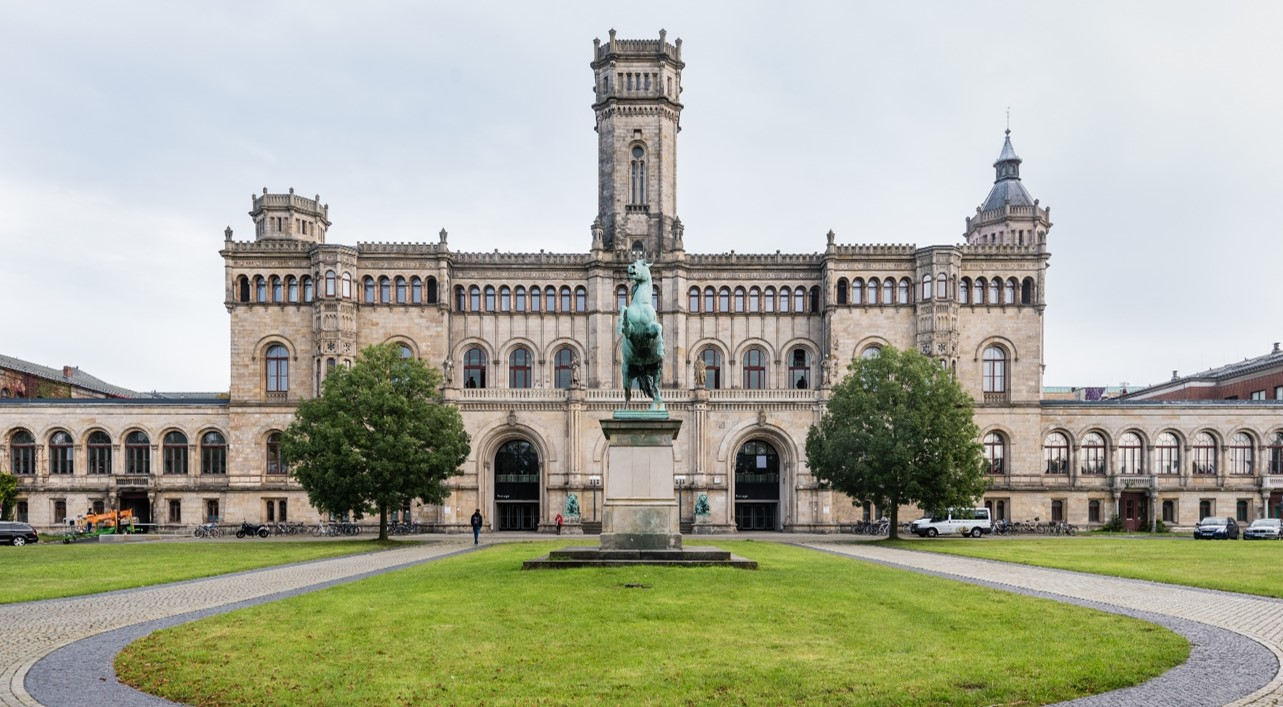
\includegraphics[width=0.65\textwidth]{figures/luh_default_presentation_title_image.jpg}}

% Title page: luhstyle
% \setbeamertemplate{title page}[luhstyle]
% % Add optional title image here
% \addtitlepageimage{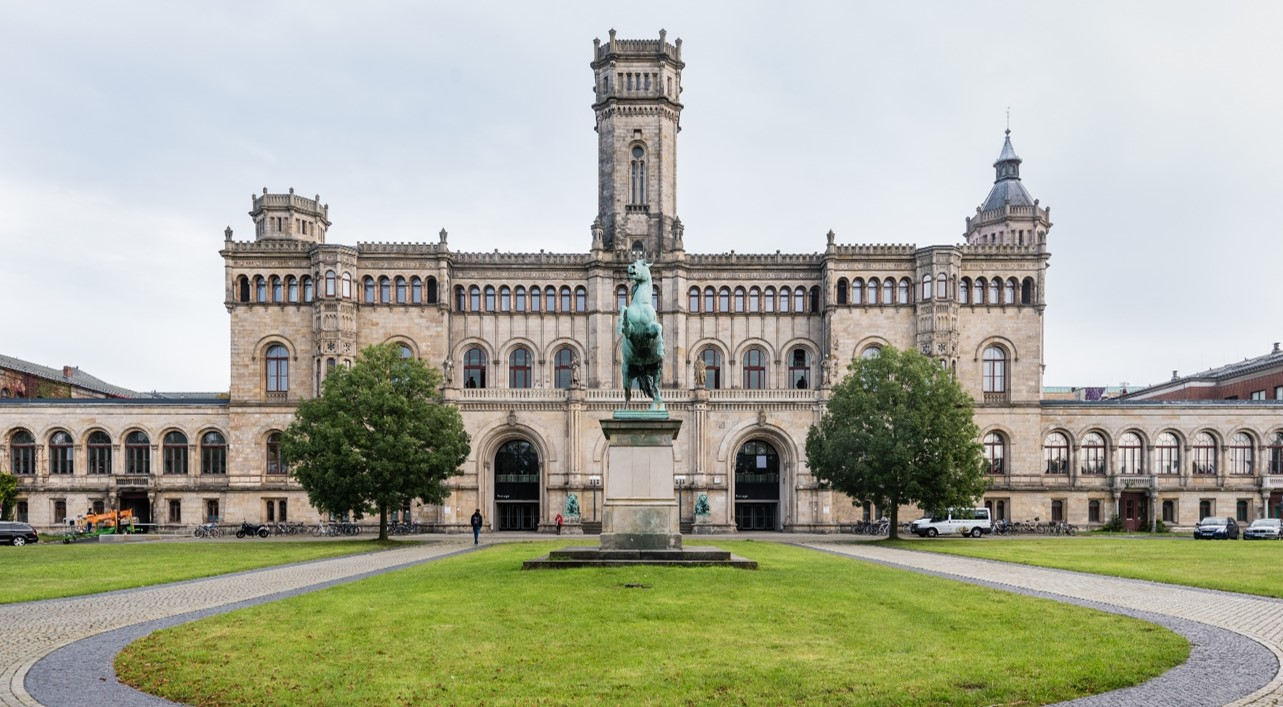
\includegraphics[width=0.75\textwidth]{figures/luh_default_presentation_title_image.jpg}}

\author[Abedjan \& Lindauer]{Ziawasch Abedjan \& Marius Lindauer\\[1em]
	
\includegraphics[height=\logoheight]{../latex_main/figures/luh_logo_rgb_0_80_155.pdf}\qquad
	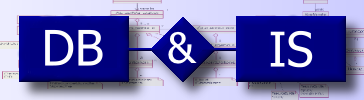
\includegraphics[height=\logoheight]{../latex_main/figures/DBIS_Kurzlogo.png}\qquad

\includegraphics[height=\logoheight]{../latex_main/figures/TNT_darkv4}\qquad

\includegraphics[height=\logoheight]{../latex_main/figures/L3S.jpg}	}
\date{Summer Term 2022; \hspace{0.5em} {
\includegraphics[height=1.5em]{../latex_main/figures/Cc-by-nc-sa_icon.svg.png}}; based on \href{https://ds100.org/fa21/}{[DS100]}
}


%%% Custom Packages
%----------------------------------------------------------------------
% Create dummy content
\usepackage{blindtext}

% Adds a frame with the current page layout. Just call \layout inside of a frame.
\usepackage{layout}


%%% Macros
%\renewcommand{\vec}[1]{\mathbf{#1}}
% \usepackage{bm}
%\let\vecb\bm

\title[Introduction]{DS: SQL}
\subtitle{Database Schemas}

\graphicspath{ {./figure/} }
%\institute{}


\begin{document}
	
	\maketitle
	\begin{frame}{Relational DBMS Terminology}
	    
	    \begin{columns}
	        \begin{column}{.75\textwidth}
	        \vspace{.4cm}\\
	        In a relational database, each table is called a relation.\\
            Each row of relation is called a record or tuple. Rows do not have names.\\
            Each column of a relation is called an attribute or field.

	                \begin{itemize}
	                    \item Attributes have names (e.g. temperature, city, legs).
	                    \item Attributes have data types (e.g. INTEGER, CHAR(20)).
	                    \item Attributes may also have constraints (e.g. must be non-negative).
	                    \item Attributes may be marked as primary or foreign keys.
	                    \begin{itemize}
	                        \item Primary key must be unique. Example on next slide.
	                        \item Foreign key means that an attribute is some other table’s primary key.
	                        \begin{itemize}
	                            \item Explicitly shows how tables are linked.
	                        \end{itemize}
	                    \end{itemize}
	                \end{itemize}
	        \end{column}
	        
	        
	        
	        \begin{column}{.25\textwidth}
	                \begin{center}
	                    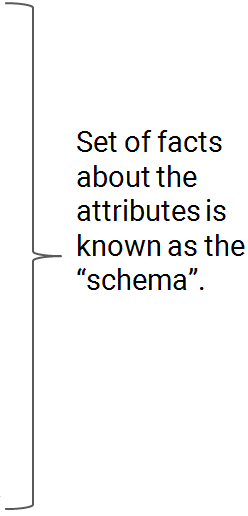
\includegraphics[scale=.35]{Bild1}
	                \end{center}
	        \end{column}
	    \end{columns}
	\end{frame}
	
	
	
	\begin{frame}{Example Relation Schema}
	    \begin{columns}
	        \begin{column}{.6\textwidth}
	             \begin{center}
	                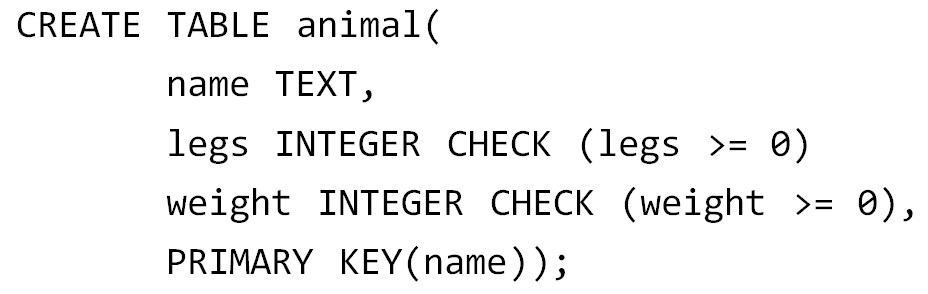
\includegraphics[scale=.35]{Bild2}
	             \end{center}
	             Given the table animal above, it is impossible to:
	             \begin{itemize}
	                 \item Insert a record with the same name as another.
	                 \item Insert a record with a negative value for legs or weight.
	                 \item Insert a record with a non-integer legs or weight.
	             \end{itemize}
	        \end{column}
	        
	        
	        
	        \begin{column}{.4\textwidth}
	                \begin{center}
	                    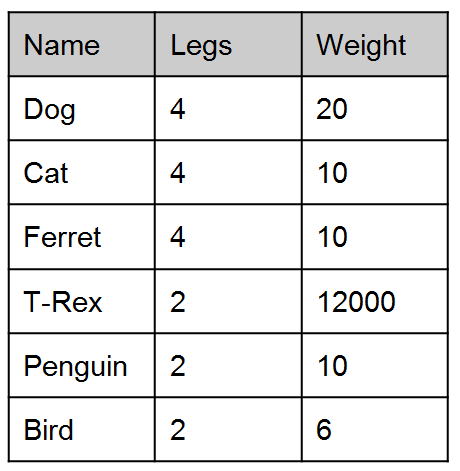
\includegraphics[scale=.35]{Bild3}
	                \end{center}
	        \end{column}
	    \end{columns}
	\end{frame}
	
	
	
	\begin{frame}[c]{Database Schema}
	    A relational database is a set of relations.
	    \begin{itemize}
	        \item Set of the schemas of those relations is called the database schema.
	        \item If the database schema includes foreign key relations, schema effectively includes a description how the tables refer to one another.
	    \end{itemize}
	\end{frame}
	
	
	\begin{frame}{Example Database Schema}
	    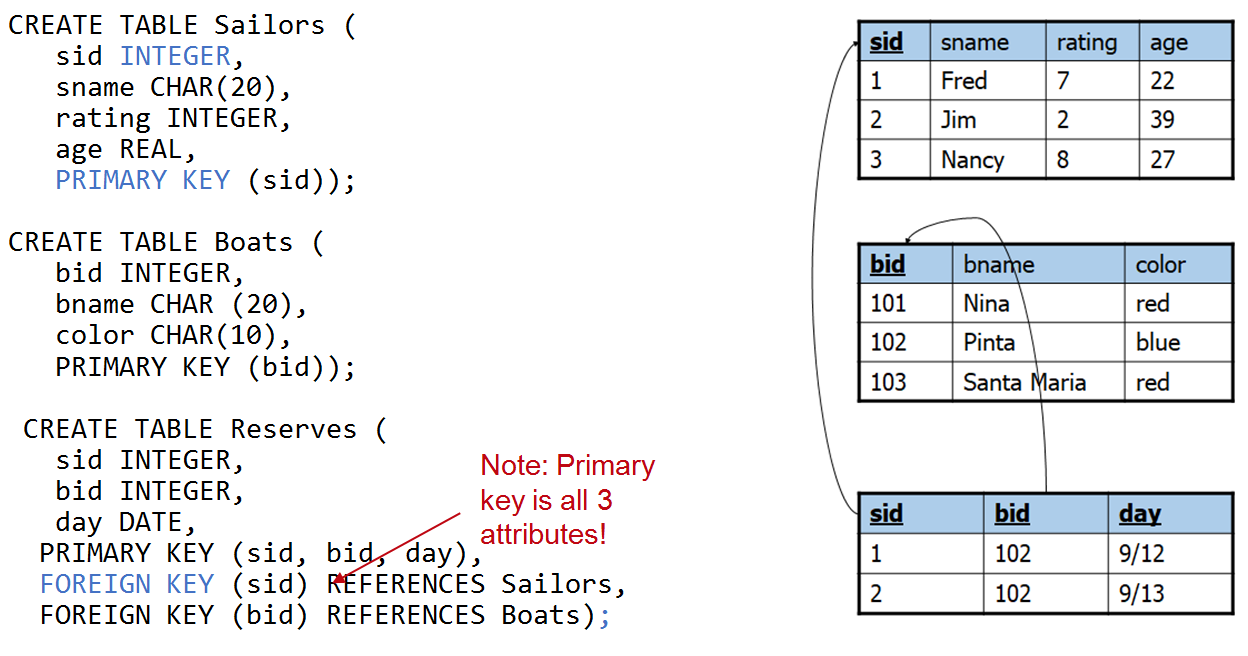
\includegraphics[scale=.4]{Bild4}
	\end{frame}
	
	
	
	
	\begin{frame}{Database Implementations}
	    We can query relational databases with SQL, but there are many implementations of SQL. 
	    \begin{itemize}
	        \item And many other database implementations that are not SQL based / relational.
	    \end{itemize}
	    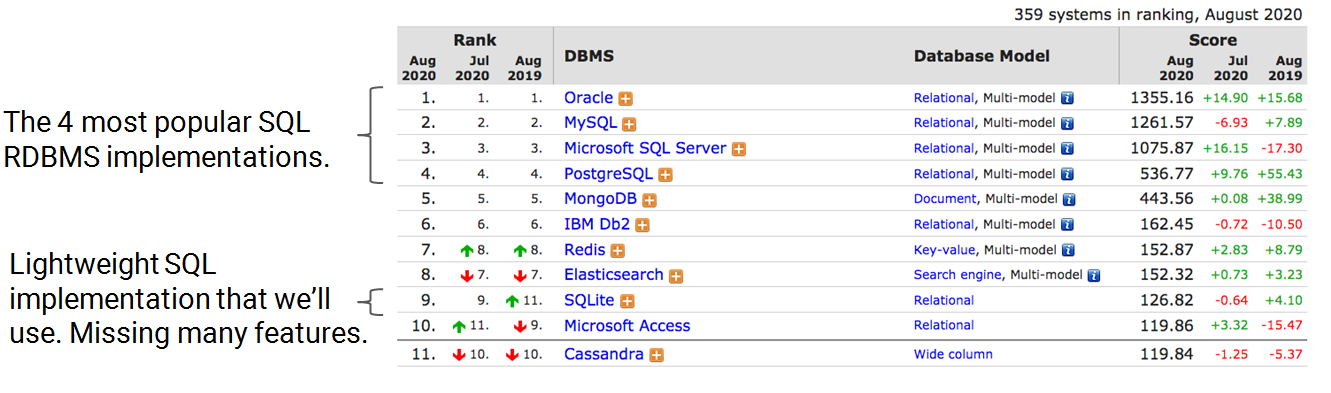
\includegraphics[scale=.4]{Bild5}\\
	    \vspace{.9cm}
	    \url{https://db-engines.com/en/ranking}
	\end{frame}
\end{document}